\section{Introduction}
\subsection{Overview}
This document identifies the architectural design specifications that satisfy the functional requirements proposed in the System Requirements Specification. It addresses the needs of the various subsystems' non-functional requirements focusing on the quality attributes, architectural patterns as well as constraints and integration requirements of the NavUP system.\newline \newline 
The following modules' designs are included in this document:
\begin{itemize}
	\item Users
	\item GIS
	\item Notification
	\item Events
\end{itemize}
The document begins with an explanation on the chosen architectural pattern and how it will be used to modularize the NavUP system. It then outlines the architectural design of each module along with all relevant UML diagrams. Finally the chosen technologies are discussed as well as the deployment of the system. 

\subsection{Architectural Pattern}
The NavUP system will be designed using the Three-tier architecture in which the user-interface, process logic and data storage are developed and maintained as independent modules. This will allow any of the three tiers to be upgraded or replaced without affecting any of the other layers. \newline
The NavUP system will be divided into 3 tiers:
\begin{itemize}
	\item Presentation tier
	\item Application tier
	\item Data tier
\end{itemize} 

\subsubsection{Presentation tier}
This is the highest level of the NavUP application. It is the layer which users will interact with directly through the user-interface. The Presentation layer will reside on the mobile and web app and will display information pulled from the Application layer in a way that is simple and intuitive to the user of the application.

\subsubsection{Application tier}
This layer resides on the application server and controls the application's functionality through detailed processing. The results of this processing is passed back to the Presentation layer which will display it to the user.

\subsubsection{Data tier}
The Data layer includes all data persistence mechanisms and resides on the database server. The application server uses this layer to manage the stored data. It is crucial that there are no dependencies on the storage mechanisms to ensure that any updates or changes will not affect the application tier clients in any way.

\pagebreak

\section{Deployment Diagram}
The diagram below depicts how the NavUP system will communicate and flow upon deployment. This can be seen as an overall view on the system in a deployment scenario.
\begin{figure}[H]
	
	\centering
	
	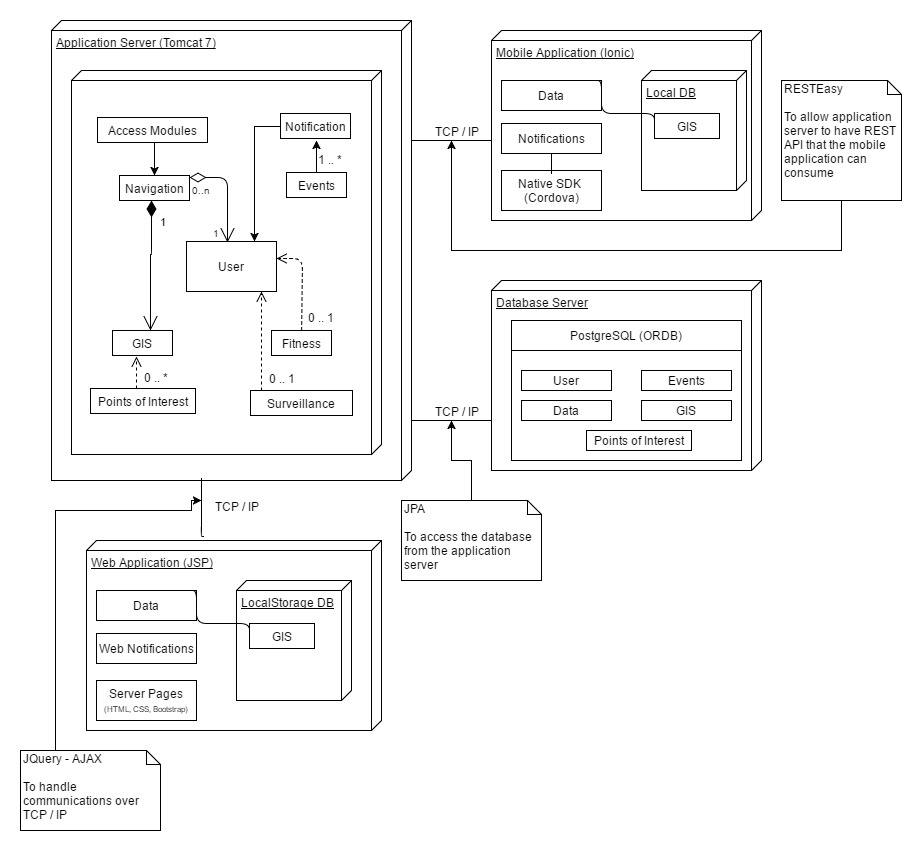
\includegraphics[width=\textwidth]{img/Deployment.jpg}
	
	\caption{NavUP Deployment Diagram}
	
	\end{figure}
\pagebreak